\documentclass{article}
% \usepackage[utf8]{inputenc}
\setlength{\parskip}{\baselineskip}%
\setlength{\parindent}{0pt}%


\title{Case Study for Insurance Modeling}
\author{Jeanne Fu}
\date{\today}

\usepackage{natbib}
\usepackage{graphicx}

\begin{document}

\maketitle

\section{Introduction}
This case study will focus on pricing strategies for a commercial auto line of business. The goal of the study is to incorporate Machine Learning to improve pricing accuracy, while maintain explainability.

Throughout the life cycle of a insurance pricing project, there are in general six steps, and we will discuss in more detail how to use ML in each step:

\begin{itemize}
    \item Scoping (Set up a goal for the project, success criteria and/or metrics, resource, cost, etc.)
    \item Data Preparation (Data sourcing, EDA, data cleaning)
    \item Feature Engineering (Transformation, variable selection)
    \item Modeling (Benchmarking, feature importance ranking, model, validation)
    \item Implementation (Deploy model for business end-users, testing)
    \item Monitoring (and prepare for model refreshing)
\end{itemize}

This case study will be focusing on Data Preparation, Modeling and Implementation. I will discuss about potential risks and how to manage them in the end.

\section{Data Preparation}
Put together both internal and external data sources, and prepare for modeling data.

Internal data source:
\begin{itemize}
    \item Policy data: account/policy information, exposure, location, primary usage of vehicle, business industry, etc.
    \item Loss data: (Target, loss history). Loss linkage may be needed. 
    \item Vehicle information: vehicle weight, vehicle age, vehicle cost, etc. May use external VIN decoding service if needed.
\end{itemize}

External data source:
\begin{itemize}
    \item Driver information (credit history, police driving record, etc.)
    \item Credit history (for the business)
\end{itemize}

Things to do:
- 
Explore missing values. 
- Check distribution


\section{Feature Engineering}

A lot of explorations could be done here. Include but not limited to:
\begin{itemize}
    \item Encoding catergorical variables
    \item Explore feature interaction
    \item Bin numerical variables, and/or explore polinomial trend
\end{itemize}



\section{Model Training and Validation}

* Split Training, Test, Holdout (or Cross Validation)

* Selection of Target variables: Frequency and Severity VS. Pure Premium

Things to think about:
\begin{itemize}
    \item Different coverages
    \item Outlier in pure premium
    \item Need to develop loss (alternative is to use policy year as control variable)
    \item Need to trend
\end{itemize}

* AutoML for model Benchmarking

* AutoML for model variable importance (Shapeley Value)

Explain what is Shapeley value 

Shapeley plot here

How to use Shapeley Plot?

\begin{itemize}
    \item Feature importance: (explain feature importance ranking)
    \item Outlier detection
    \item 
    \item 
\end{itemize}

% \begin{figure}[h!]
% \centering
% 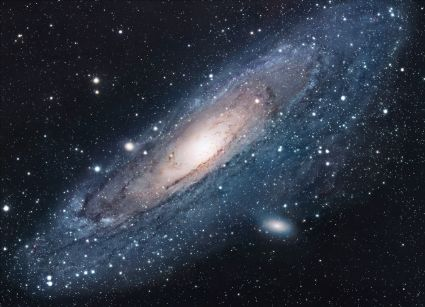
\includegraphics[scale=1.7]{universe.jpg}
% \caption{The Universe}
% \label{fig:univerise}
% \end{figure}

\section{Potential Risks and How to Manage Them}



\section{Conclusion}
% ``I always thought something was fundamentally wrong with the universe'' \citep{adams1995hitchhiker}

\bibliographystyle{plain}
\bibliography{references}
\end{document}
